\subsection{The fabrication is the objective, not the network}
A natural objection is that our generative baseline is a straw man. It is not: it is
the \emph{perception-optimal} endpoint of a real tradeoff. We train the \emph{same}
1-D CNN with a distortion-to-perception sweep (MSE plus an adversarial term of weight
$\lambda$) and score each with the certificate (Fig.~\ref{fig:pd}). At $\lambda{=}0$
(distortion-optimal) the trained network behaves like OLS: its non-dipolar energy is
\emph{correlated} with truth ($\rho{=}{+}0.24$)---it recovers genuine Tier~II and does
not fabricate. The moment realism enters the objective the correlation collapses
($\rho{\approx}0$ for every $\lambda{>}0$) while the hallucination energy climbs (to
$h{=}0.30$\,mV at $\lambda{=}2$) and distortion worsens---the perception-distortion
tradeoff \cite{blau2018perception} on the ECG. Fabrication is a property of the
\emph{objective}, not of using a network, and the certificate measures it directly.

\begin{figure}[t]
  \centering
  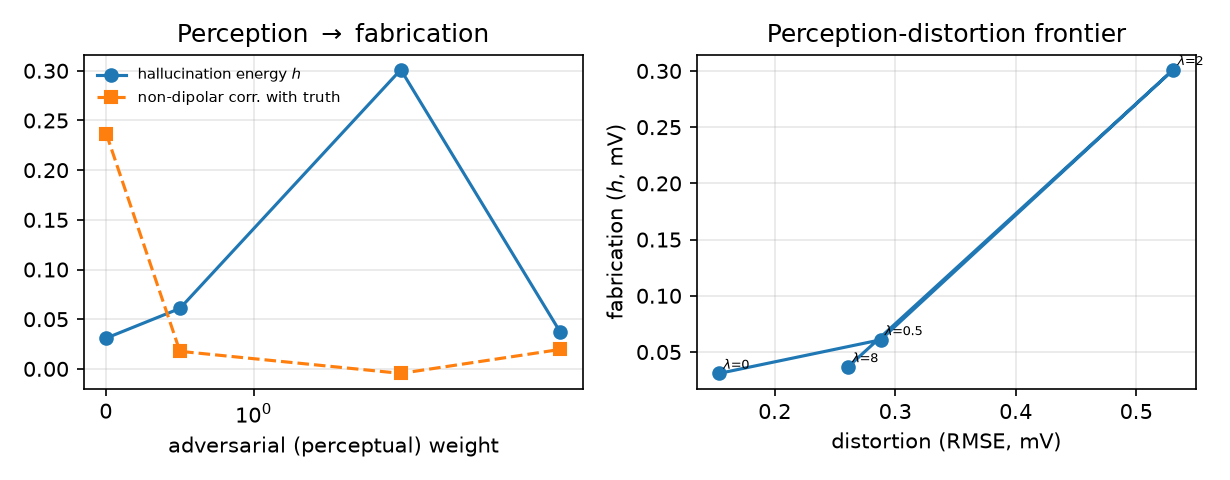
\includegraphics[width=\linewidth]{../results/neural_perception_distortion.png}
  \caption{A single trained CNN swept from distortion- ($\lambda{=}0$) to
  perception-optimal. The instant any realism enters the objective the non-dipolar
  correlation with truth collapses ($\rho{:}{+}0.24{\to}{\approx}0$ for every
  $\lambda{>}0$); certified hallucination energy climbs into the perceptual regime
  (peak $h{=}0.30$\,mV at $\lambda{=}2$). Fabrication is chosen by the objective.}
  \label{fig:pd}
\end{figure}
